\section{The pass@1 price}
\label{sec:price}

This section proves the two central results. Probability on the strategy simplex
is a conserved quantity: raising it on one strategy lowers it on another. When
strategies specialize, that accounting is visible at the level of prompts, and
it is the source of the pass@$k$ crossover. We state each result, give the
argument, and report the numbers produced by the package; full proofs are in the
appendix.

\subsection{No free lunch}
\label{sec:nfl}

Probability on the strategy simplex is conserved: a unit added to one strategy
is a unit removed from another. When strategies specialize, that single
accounting fact becomes a hard constraint on what reinforcement can buy. We make
it exact.

Fix an interior policy $w$ and a tangent $\mathrm{d}w$ with
$\mathbf{1}^{\top}\mathrm{d}w=0$. A \emph{free lunch} is a $\mathrm{d}w$ with
$Q\,\mathrm{d}w\ge0$ and $Q\,\mathrm{d}w\ne0$; since
$\inner f{\mathrm{d}w}=\tfrac1N\mathbf 1^\top Q\,\mathrm{d}w$, it is a pass@1 gain
with no prompt regressing, and its existence does not depend on $w$.

\paragraph{Exact condition (Theorem \ref{thm:nfl}(a)).}
The feasible non-regressing directions form the cone
$K=\{\mathrm{d}w:\;Q\,\mathrm{d}w\ge0,\ \mathbf 1^\top\mathrm{d}w=0\}$, and a free
lunch is a point of $K$ with $Q\,\mathrm{d}w\ne0$. Parameterizing $K$ by a basis
of the tangent space and applying Stiemke's lemma, no such direction exists iff
there is a strictly positive $y\in\R^N_{>0}$ with $Q^\top y\perp$ the tangent
space, i.e.\ $Q^\top y=\mu\mathbf 1$: a strictly positive reweighting of prompts
equalizing strategy fitness. Because $f=\tfrac1N\sum_x q_x$, this is equivalent
to the inhomogeneous form \eqref{eq:farkas} with $y'\ge0$; we use the Stiemke
form, whose strict positivity is the right object.

\paragraph{When it holds (Theorem \ref{thm:nfl}(b,b$'$)).}
Being the \emph{unique best} on a set is not enough: Proposition
\ref{prop:uniquebest} exhibits a unique-best instance with a free lunch, where a
near-generalist absorbs the defunded mass. What suffices is \emph{exclusivity}.
Under Assumption \ref{ass:spec}, any $\mathrm{d}w$ with $\mathrm{d}w_j<0$ (one
exists whenever $\mathrm{d}w\ne0$) strictly lowers every prompt in
$X_j^{\mathrm{excl}}$, since only $j$ solves them; so no non-regressing direction
moves mass, and every pass@1 gain lowers some prompt. The realistic
$\varepsilon$-version (b$'$) follows by a Neumann-series construction of a strictly
positive price on representative prompts (appendix). Part (c) is immediate.

\paragraph{Verification.}
The Stiemke primal and dual agree in $100\%$ of instances across six generators
(exclusive, unique-best, quasi-generalist, overlapping, near-generalist,
dominant), confirming (a). Exclusive specialization gives no free lunch in
$1000/1000$ and dominant specialization in $2000/2000$. The hypothesis is sharp:
the unique-best counterexample of Proposition \ref{prop:uniquebest} has a free
lunch of $+0.173$ with the Stiemke dual infeasible, and an adversarial
near-generalist generator produces a free lunch in $500/500$ instances. Unique
best is insufficient; exclusivity, or dominance with margin, is what the price
requires.

\subsection{The pass@k price}
\label{sec:passkprice}

Write $G=F_\tau-F_0$ for the difference of the per-prompt success CDFs and
$\Delta_k=\PassK_k(\wt)-\PassK_k(\wz)$. Integrating by parts,
\begin{equation}
\label{eq:deltak}
\Delta_k=-k\int_0^1 (1-p)^{k-1}\,G(p)\,\mathrm{d}p
        =-k\int_0^\infty e^{-(k-1)s}\,G(1-e^{-s})\,\mathrm{d}s,
\qquad s=-\log(1-p).
\end{equation}

\paragraph{Argument for Theorem \ref{thm:price}.}
The kernel in \eqref{eq:deltak}, $k\mapsto e^{-(k-1)s}$, is totally positive of
all orders in $(k,s)$; by Karlin's variation-diminishing property the map
$k\mapsto\Delta_k$ has at most as many sign changes as the single-variable
function $G$, which gives (a). For (b) we place mass at success levels whose
$s$-values are geometrically spread and alternate the sign of the shift, so that
each crossing dominates its own decade of $k$; a mass-conserving alternating
shift at $n$ levels realizes $\Svar(G)=n-2$ crossings. For (c), Assumption
\ref{ass:spec} forces a per-prompt loss and Assumption \ref{ass:fine} routes it
to the minimal-success prompt: since every strategy covering it has
$f_j<R_0\le\Lambda(\tau)/\tau$, all lose mass and $\min_x p_x$ strictly drops, so
$G>0$ near $p=0$ and by \eqref{eq:deltak} the large-$k$ integral makes
$\Delta_k<0$. Part (d) is the order-preserving case: a monotone $\phi$ makes $G$
change sign at most once, so \eqref{eq:deltak} inherits at most one crossing; this
recovers the single crossover of the function case \citep{yangchen2026kernel} and
extends it to the kernel case their Remark~1 leaves open. Part (e) is Assumption
\ref{ass:fine} failing: if the hard tail keeps a high-fitness backup, the loss
does not reach it and no crossover forms.

\begin{corollary}[No reasoning for free]
\label{cor:noreasoning}
Under Assumptions \ref{ass:spec} and \ref{ass:fine}, every pass@1-improving RLVR
update is overtaken by the base model at large $k$: there is no update that
raises pass@1 and dominates the base pass@$k$ curve for all $k$. Reinforcement
cannot widen the pass@$k$ frontier; it can only move along it. This is the exact
sense in which RLVR does not add reasoning capacity beyond the base model (cf.\
Yue et al., 2504.13837); Theorem \ref{thm:price}(e) shows the conclusion is
tight, failing precisely when Assumption \ref{ass:fine} does.
\end{corollary}

\begin{figure}[t]
\centering
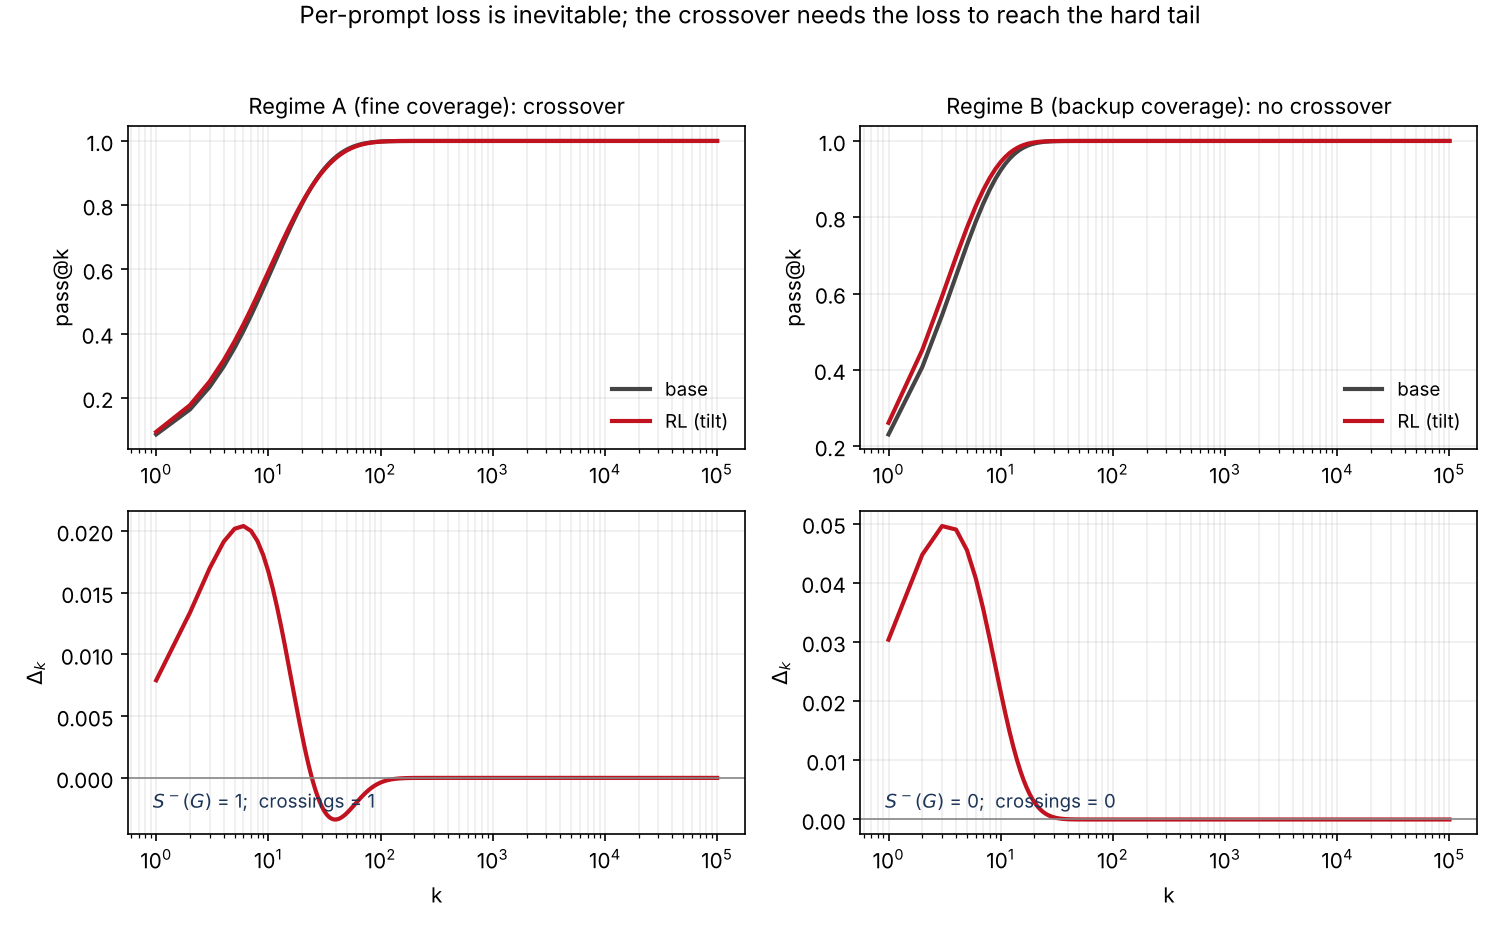
\includegraphics[width=\linewidth]{fig2_regimes.png}
\caption{Per-prompt loss is inevitable under specialization, but the aggregate
pass@$k$ crossover is conditional on Assumption \ref{ass:fine}. Regime A (fine
coverage) has a genuinely hard tail that the tilt starves, so $\Delta_k$ turns
negative and the curves cross; $\Svar(G)=1$ and the single crossing saturates
the bound. Regime B gives every prompt backup coverage, so the hard tail keeps a
floor, $\Delta_k$ stays nonnegative, and there is no crossover. Both regimes have
a per-prompt loss; only A has an aggregate crossover.}
\label{fig:regimes}
\end{figure}

\paragraph{Verification.}
The bound (a) is never violated on $3000$ random instances, and (b) is attained:
configurations with exactly $1,2,\dots,6$ crossings are constructed. Uniqueness
(d) holds in $1035/1035$ order-preserving instances. The conditional nature of
(c) is sharp (Figure \ref{fig:regimes}): when fine coverage holds the hardest
prompt's success drops and an aggregate crossover appears in $400/400$ instances;
when it fails (the hard tail keeps a high-fitness backup) neither the minimum
drops nor a crossover forms, in $0/400$.

\subsection{The price frontier}
\label{sec:frontier}

The crossover is not an avoidable artifact: it is the aggregate shadow of the
per-prompt price, and any attempt to remove it pays in pass@1. We make the
exchange rate exact. For $\gamma\in[0,1]$, let $w(\gamma)$ solve
\begin{equation}
\label{eq:frontierlp}
\max_{w\in\Delta^{M-1}}\ \inner{w}{f}
\quad\text{s.t.}\quad p_x(w)\ge\gamma\,p_x(\wz)\ \ \text{for all } x,
\end{equation}
a linear program in $Q$: raise pass@1 while letting no prompt fall below a
fraction $\gamma$ of its base success.

The map $\gamma\mapsto(\text{pass@1 gain},\,\text{worst pass@}k\text{ loss})$ it
traces is Theorem \ref{thm:frontier}: monotone, with the unconstrained GRPO point
at $\gamma=0$ and, at $\gamma=1$, first-order stochastic dominance $F_\tau\le F_0$
hence $\Delta_k\ge0$ for all $k$, which under Assumption \ref{ass:spec} forces
zero pass@1 gain.

\begin{figure}[t]
\centering
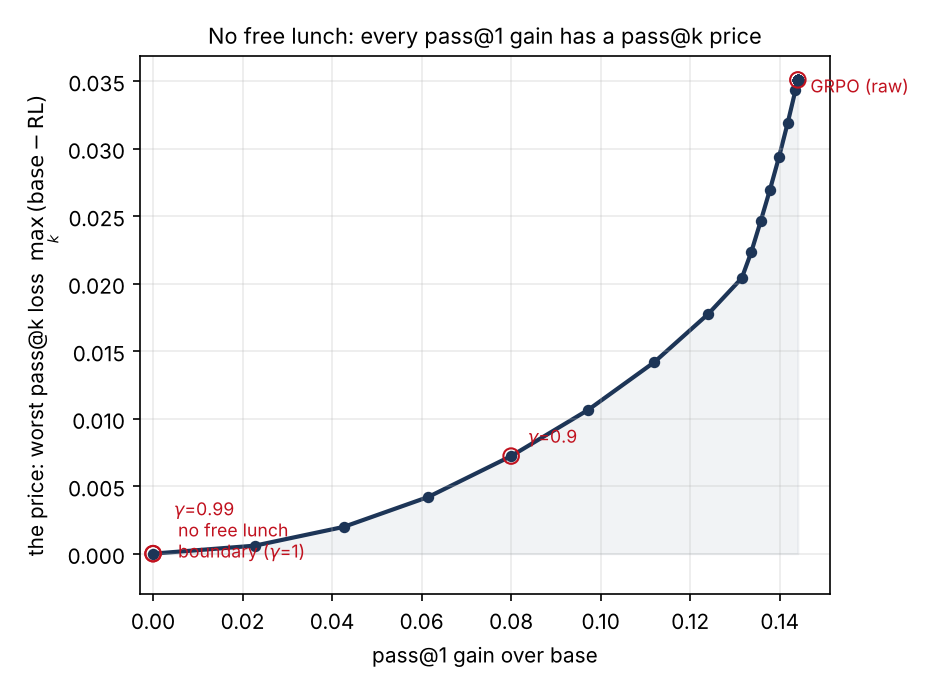
\includegraphics[width=0.66\linewidth]{fig1_price_frontier.png}
\caption{The no-free-lunch frontier. Each point is the best pass@1 gain
achievable at a given per-prompt floor $\gamma$, against the price it pays, the
worst pass@$k$ loss $\max_k(\mathrm{base}-\mathrm{RL})$. The unconstrained GRPO
update (top right) buys the largest gain at the largest price; tightening
$\gamma$ slides down the curve; $\gamma=1$ reaches the origin, where the only
way to pay nothing is to gain nothing (Theorem \ref{thm:frontier}). The curve is
the exchange rate; its slope is the marginal price of a unit of pass@1.}
\label{fig:frontier}
\end{figure}

\paragraph{Verification.}
At $\gamma=1$ the constrained update gives zero crossings and first-order
dominance in $400/400$ instances, with the worst per-prompt loss at machine zero
and zero median pass@1 gain: no free lunch, exactly. As $\gamma$ decreases the
pass@1 gain rises monotonically and the crossing moves to smaller $k$ (Figure
\ref{fig:frontier}). The frontier is thus a strict trade: there is no setting
that both improves pass@1 and removes the crossover. The ``correction'' is the
frontier itself, not an escape from it.